The goodness of the fit (GOF) indicates how well the model PDF (probability
distribution function) agrees with the data. There are various algorithms to
compute the GOF such as {\bf{saturated}} (Baker-Cousins)~\cite{Baker:1983tu}, KS
(Kolmogorov-Smirnov)~\cite{ks1},~\cite{smirnov1948}, and
AD (Anderson-Darling)~\cite{anderson1952}. The saturated algorithm is used in this analysis
for GOF. The test statistics as a measure of GOF is given as \cite{Baker:1983tu}
\begin{equation}
q_{GoF, saturated} = -2\ln \left(\frac{L_{nominal} (n|\mu s(\theta) + b(\theta))}{L_{saturated}(n|n)}\right)
\label{eq:gof}
\end{equation}

The likelihood functions of Eq.~\ref{eq:gof} are given by
\begin{equation}
L_{nominal} (n|\mu s(\theta) + b(\theta)) = \prod_{j=1}^N \frac{(\mu s_j(\theta) + b_j(\theta))^{n_j}}{n_{j}!} \exp(-(\mu s_j(\theta) + b_j(\theta)))
\label{eq:lNominal}
\end{equation}
and,
\begin{equation}
L_{saturated} (n|n) = \prod_{j=1}^N \frac{(n_j)^{n_j}}{n_{j}!} \exp(-n_j)
\label{eq:lSaturated}
\end{equation}


Where, $n_j$ is the expectation value in $j^{th}$ bin of data, N is the total number of bins. The
$s_j(\theta)$ and $b_j(\theta)$ are mean number of events in $j^{th}$ bin of signal and background
process and depend on the nuisance parameters ($\theta$). The $\mu$ is the signal strength which is
zero for background only hypothesis and non-zero for signal+background hypothesis. In $j^{th}$ bin,
$s_j(\theta)$ and $b_j(\theta)$ are given by \cite{Cowan:2010js}

\begin{equation}
s_{j}(\theta) = s_{tot}\int_{j^{th} bin} f_s(x; \theta_s)dx,
\end{equation}

\begin{equation}
b_{j}(\theta) = b_{tot}\int_{j^{th} bin} f_b(x; \theta_b)dx.
\end{equation}
The $f_s(x; \theta_s)$ and $f_b(x; \theta_b)$ are PDFs for signal and background events.
The $s_{tot}$ and $b_{tot}$ are mean of total number of events from signal and background process.

Using Eq.~\ref{eq:lNominal}, and Eq.~\ref{eq:lSaturated},
\begin{equation}
q_{GoF, saturated} = 2\sum_{j}\left(\mu s_j(\theta) + b_j(\theta) - n_j + n_j\ln\left(\frac{n_j}{\mu s_j(\theta) + b_j(\theta)}\right)\right)
\label{eq:gofFinal}
\end{equation}

The goodness of fit ($q_{GoF, saturated}$) is shown in Figure~\ref{fig:GOF} for lepton channel from
exclusive charm categories for all signal mass points using observed data and toys MC. Lower the
value of GOF, the better is the agreement between data and model PDF. For different channels and
various event categories, the GOF is linearly added over different bins, which can be seen from
different columns of Tables~\ref{tab:gofMu},~\ref{tab:gofEle}, and \ref{tab:gofLep}. 
The GOF is performed using the Command (\ref{cmd:GOF}).
\begin{figure}
    \centering
    \subfigure[]{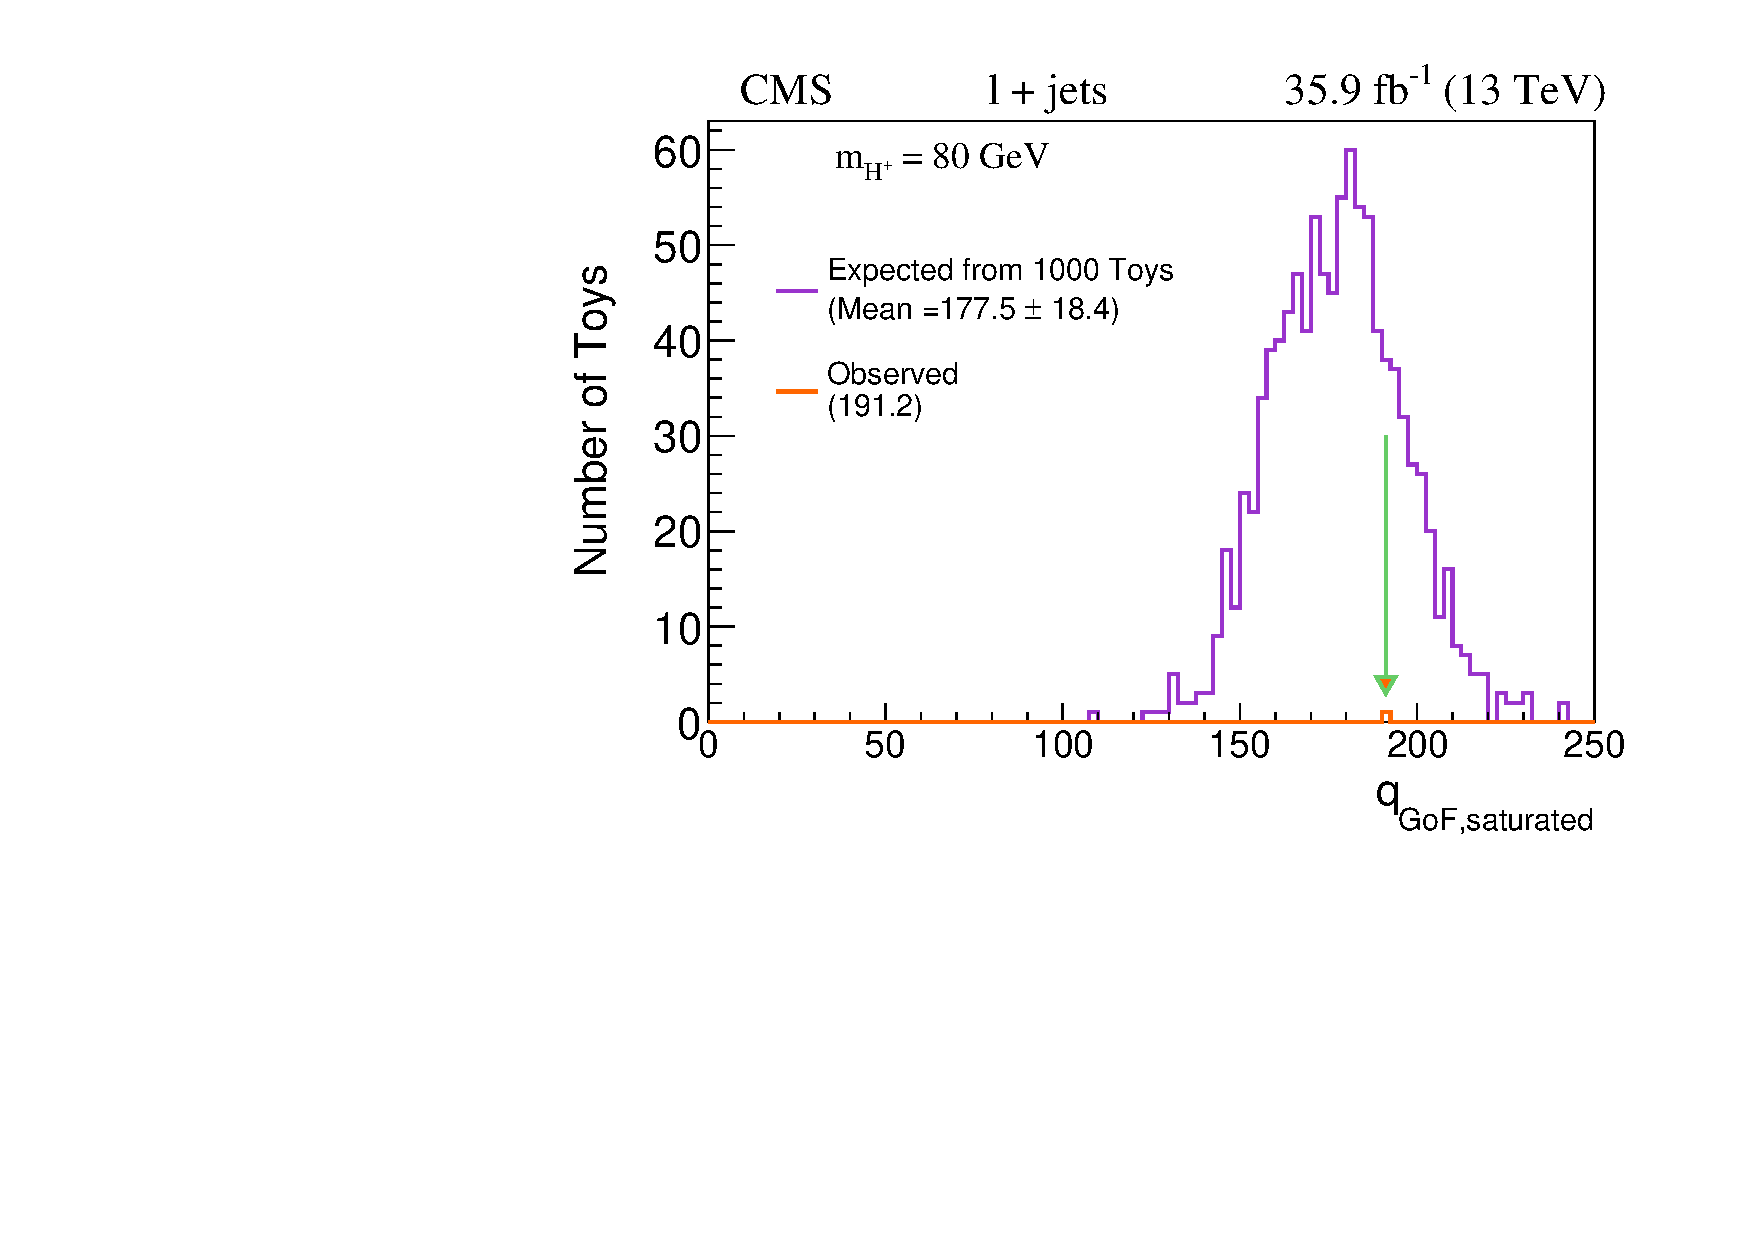
\includegraphics[width=0.45\linewidth]{Image/GOF/GOF_mu_ele_Cat3_cTagEx_80.pdf}}
    \subfigure[]{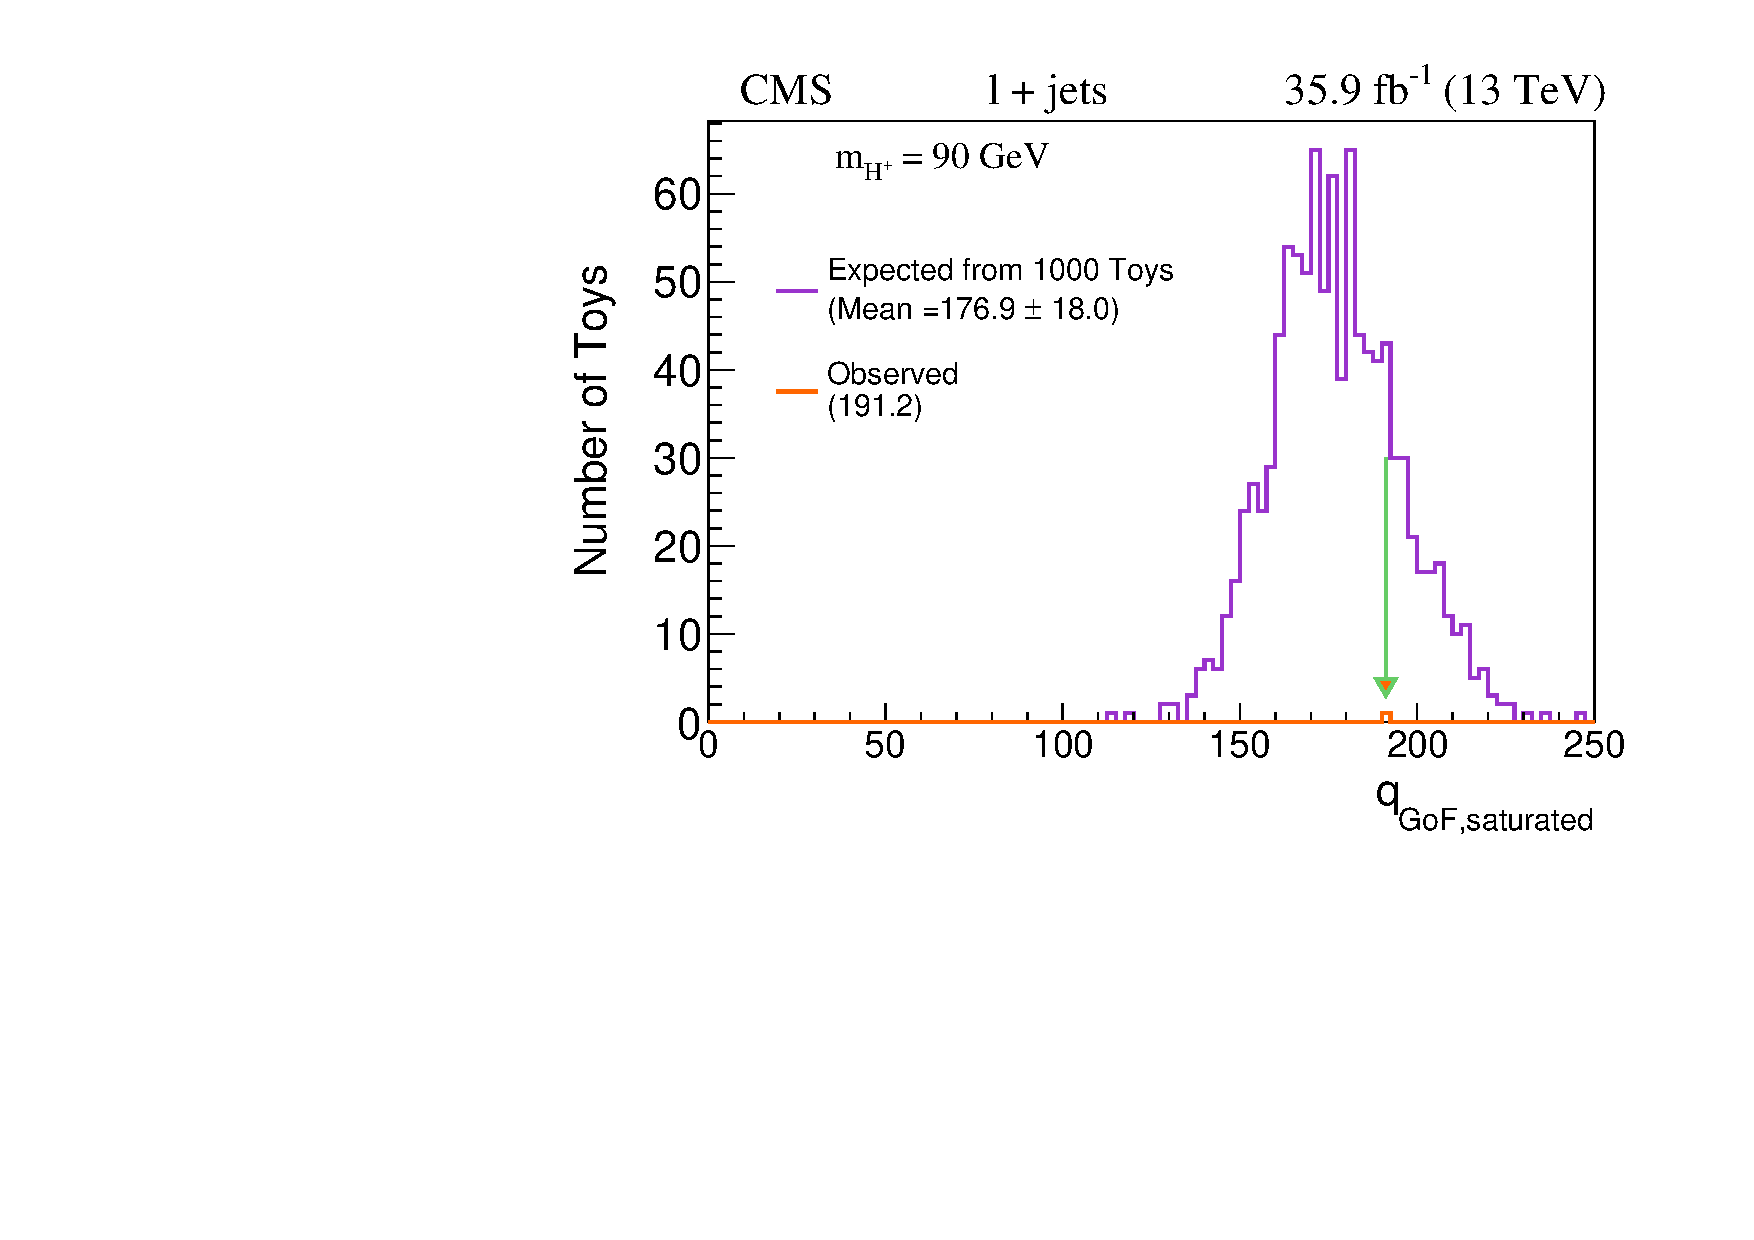
\includegraphics[width=0.45\linewidth]{Image/GOF/GOF_mu_ele_Cat3_cTagEx_90.pdf}}
    \vfil
    \subfigure[]{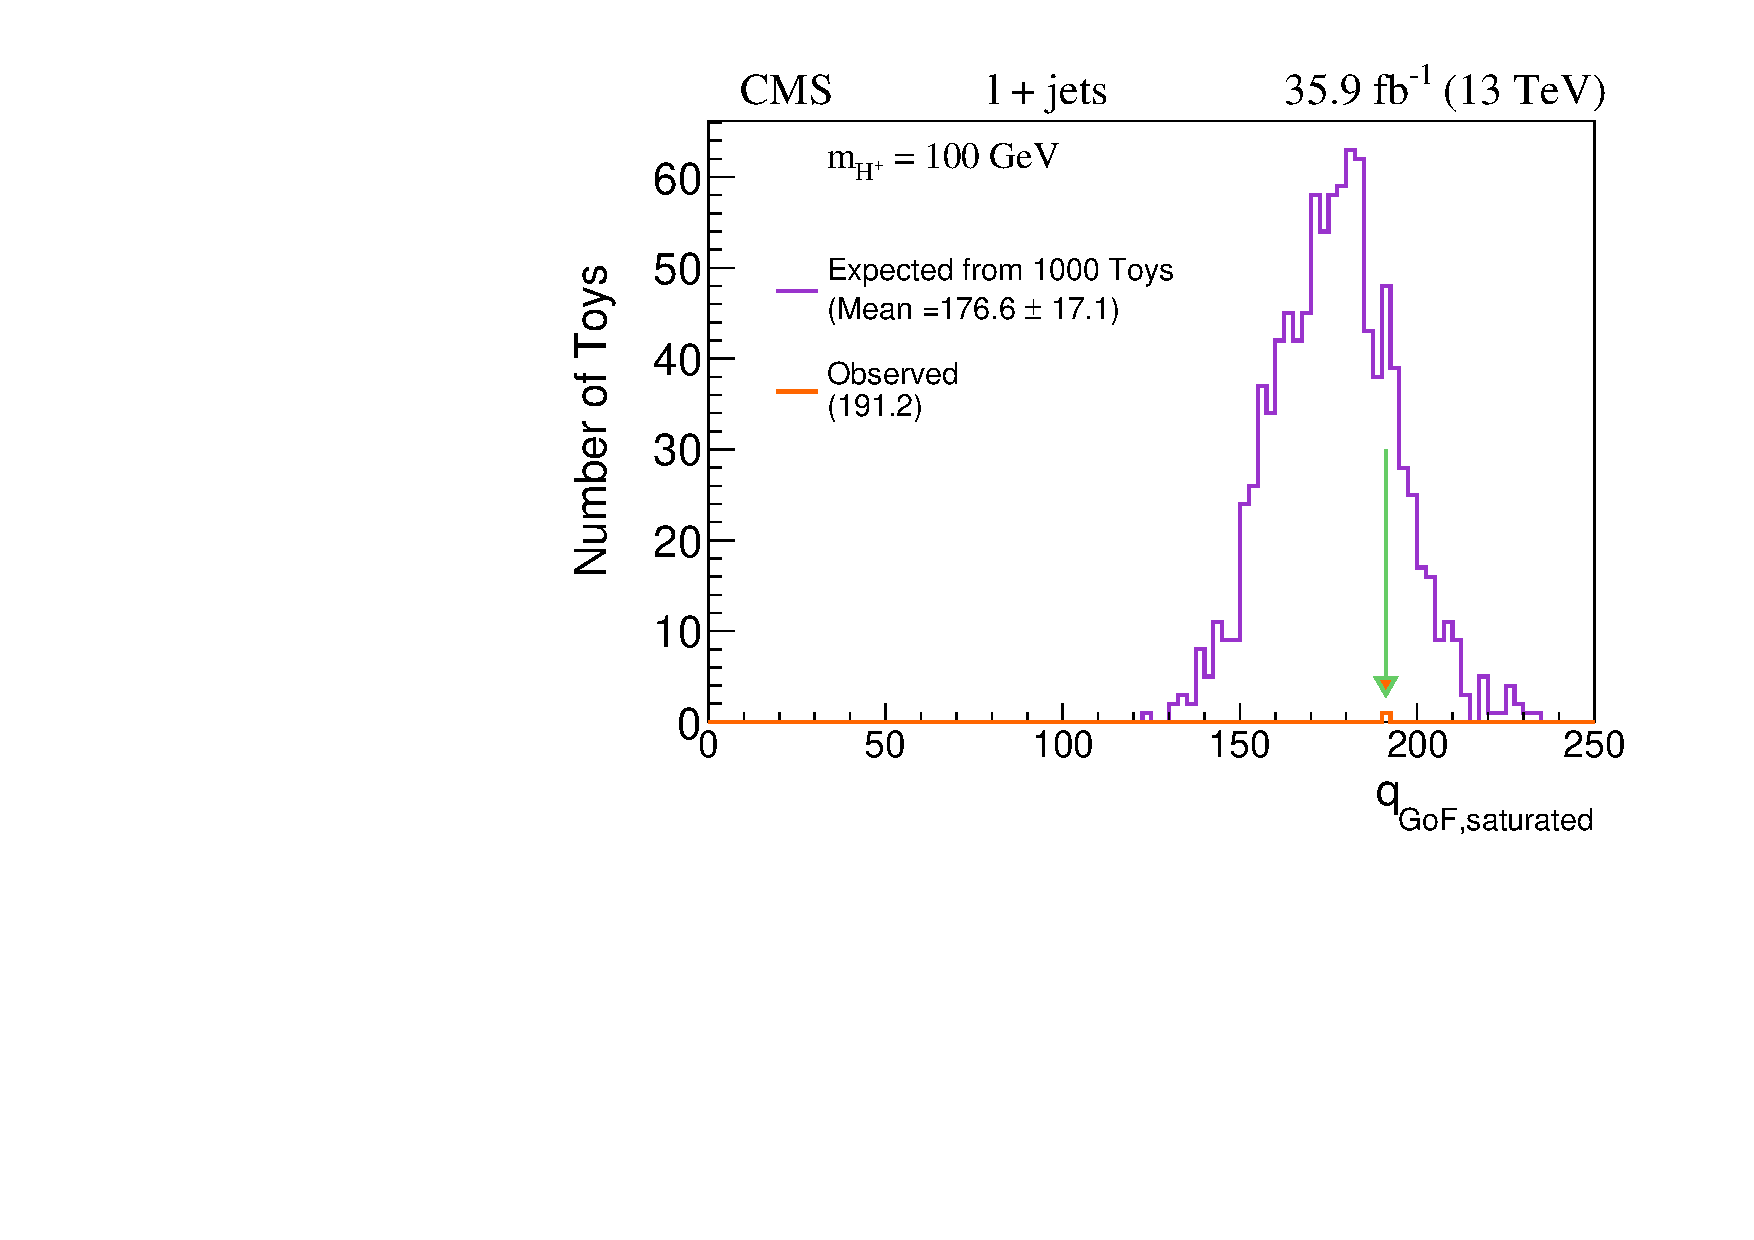
\includegraphics[width=0.45\linewidth]{Image/GOF/GOF_mu_ele_Cat3_cTagEx_100.pdf}}
    \subfigure[]{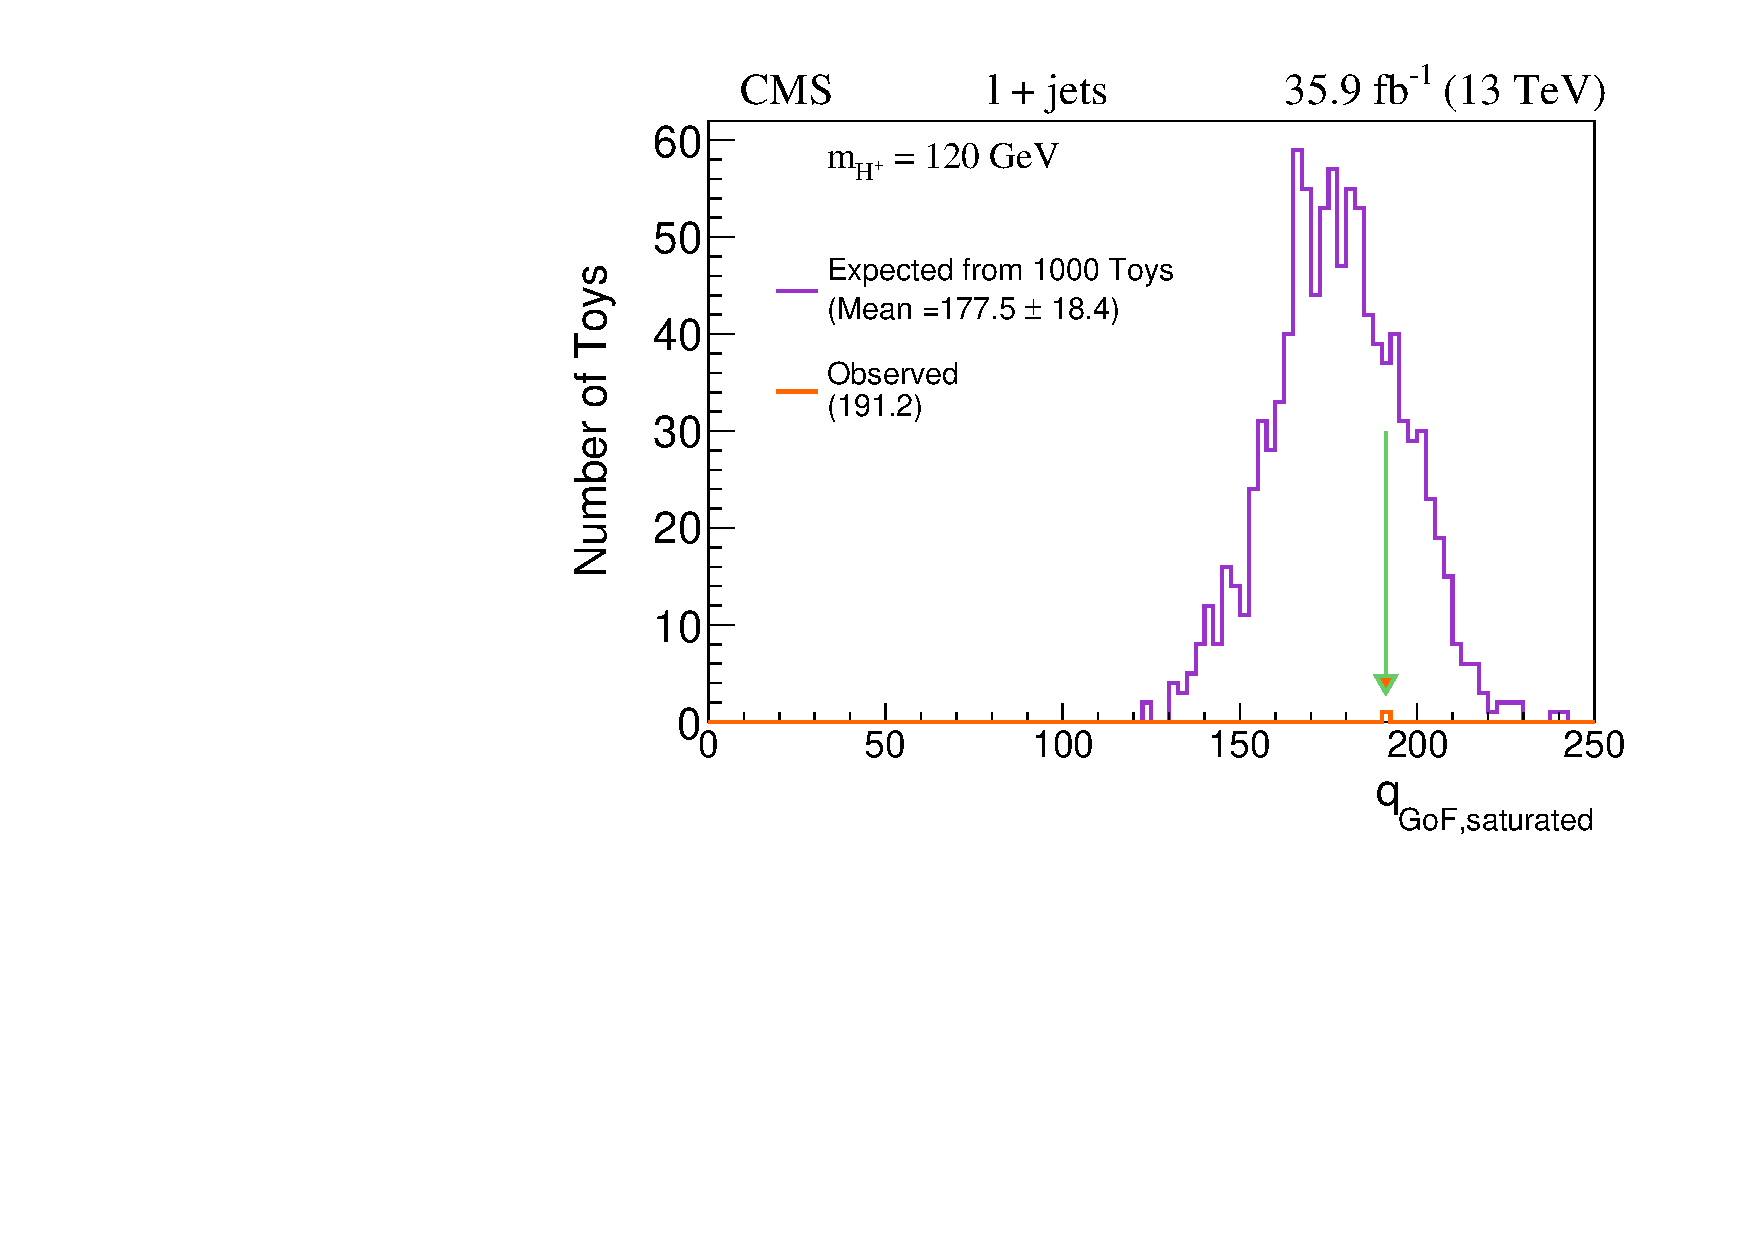
\includegraphics[width=0.45\linewidth]{Image/GOF/GOF_mu_ele_Cat3_cTagEx_120.pdf}}
    \vfil
    \subfigure[]{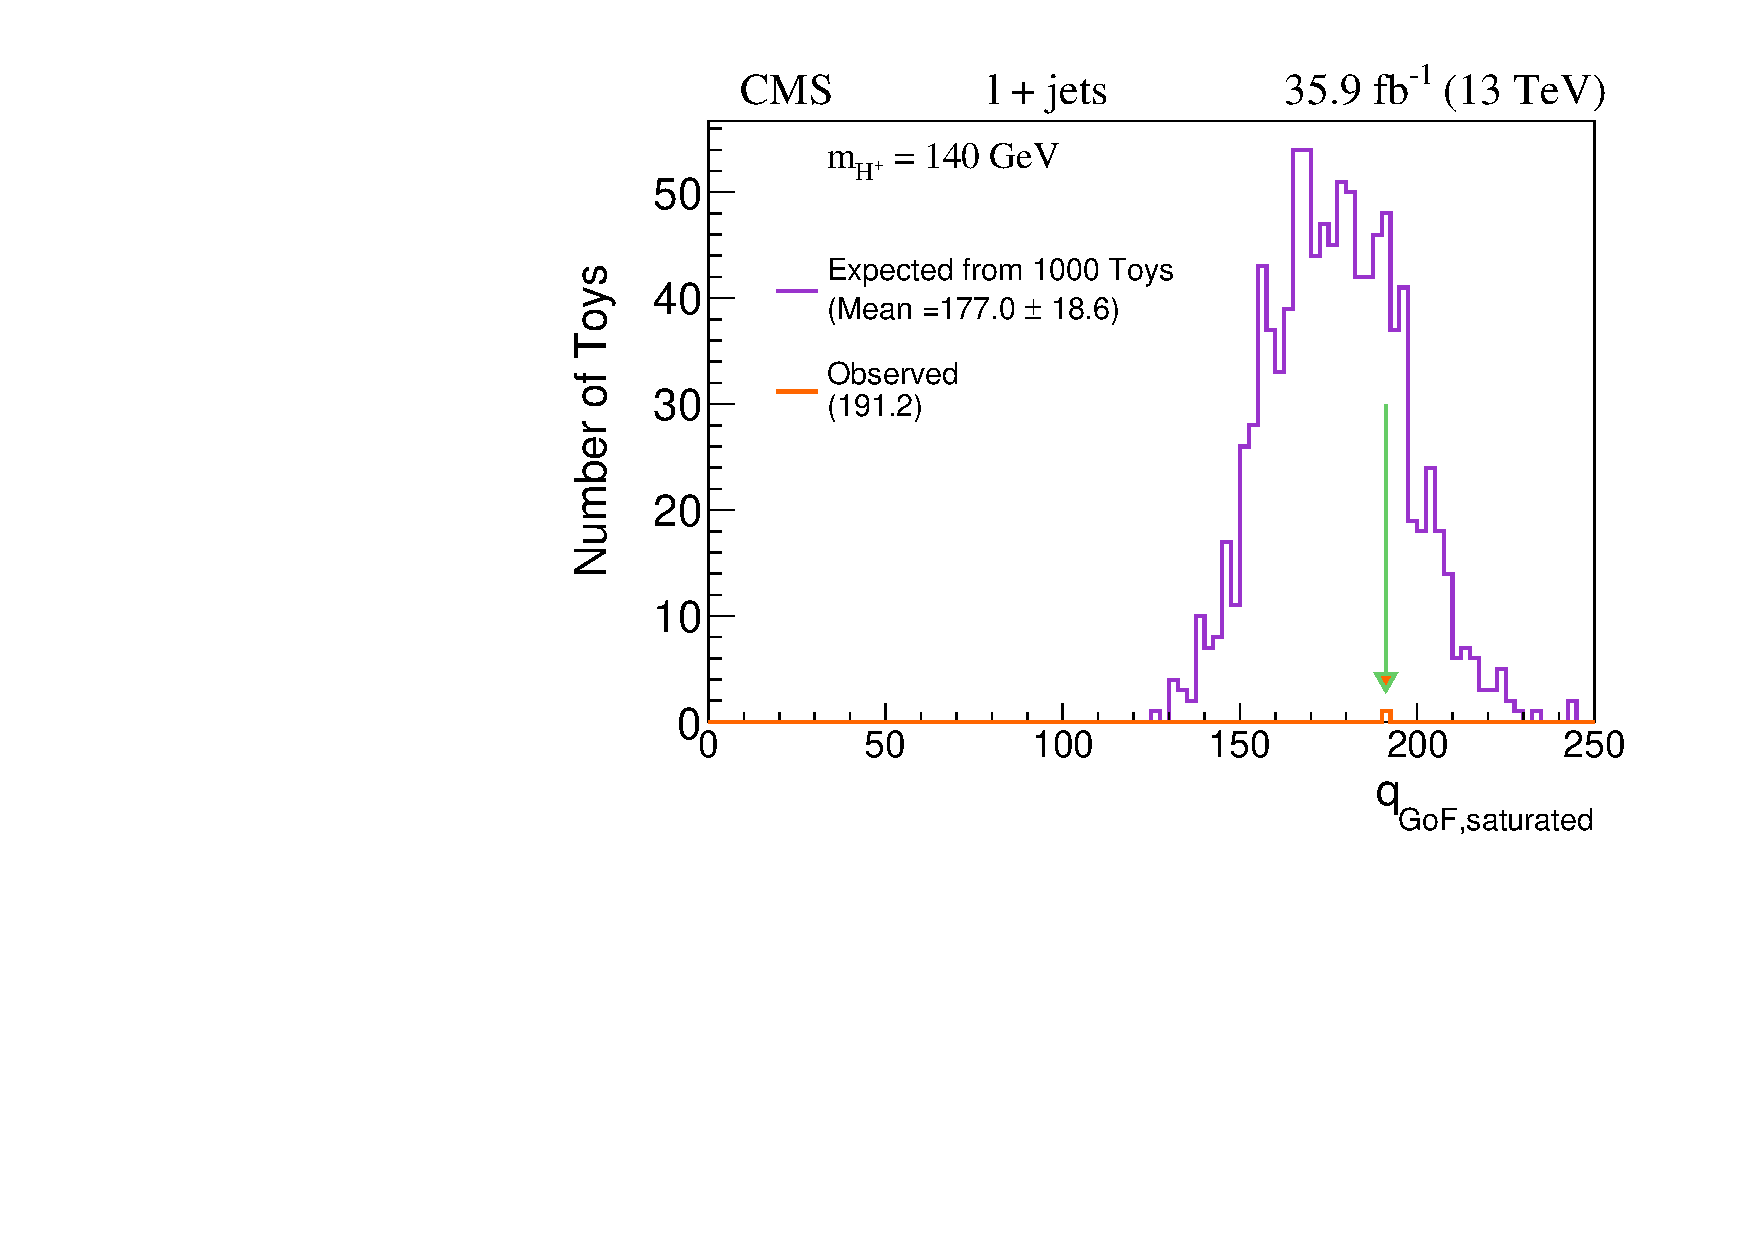
\includegraphics[width=0.45\linewidth]{Image/GOF/GOF_mu_ele_Cat3_cTagEx_140.pdf}}
    \subfigure[]{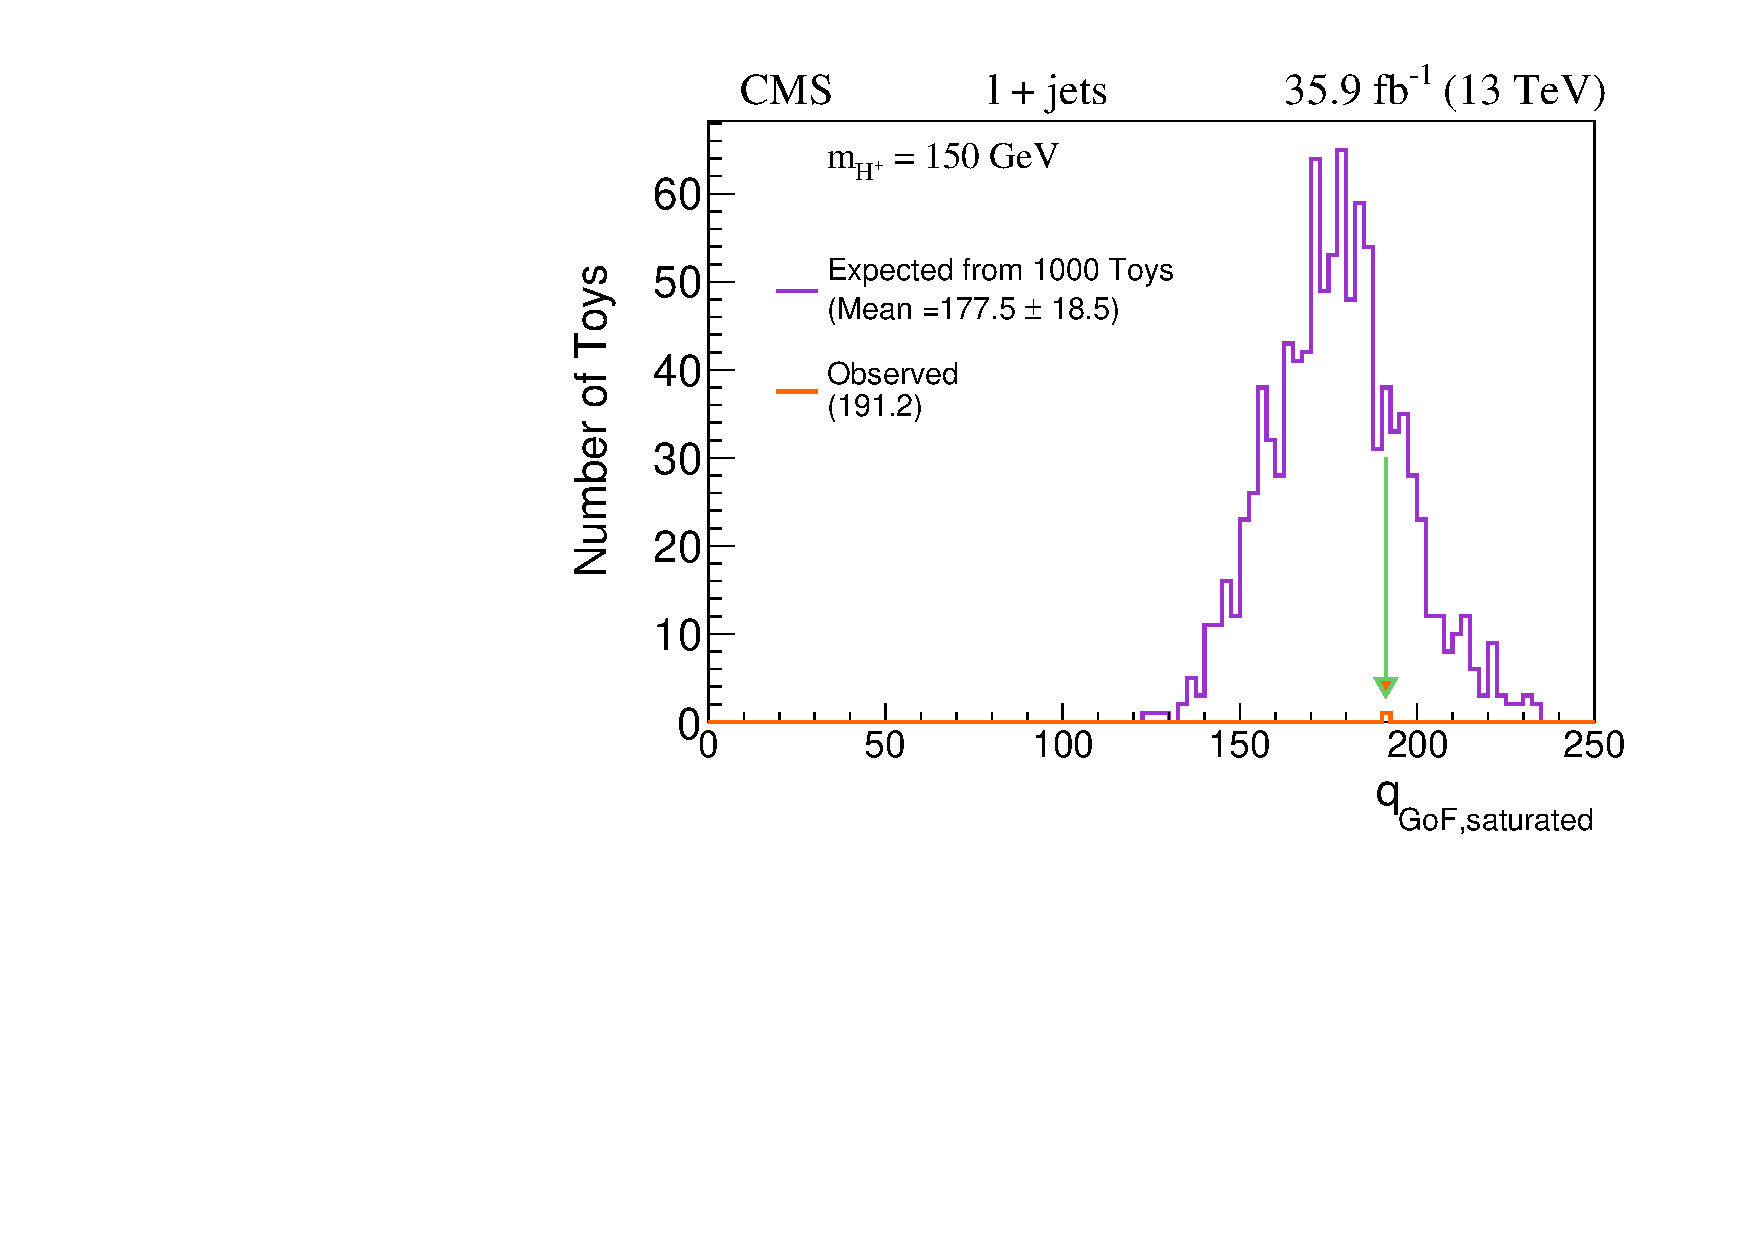
\includegraphics[width=0.45\linewidth]{Image/GOF/GOF_mu_ele_Cat3_cTagEx_150.pdf}}
    \vfil
    \subfigure[]{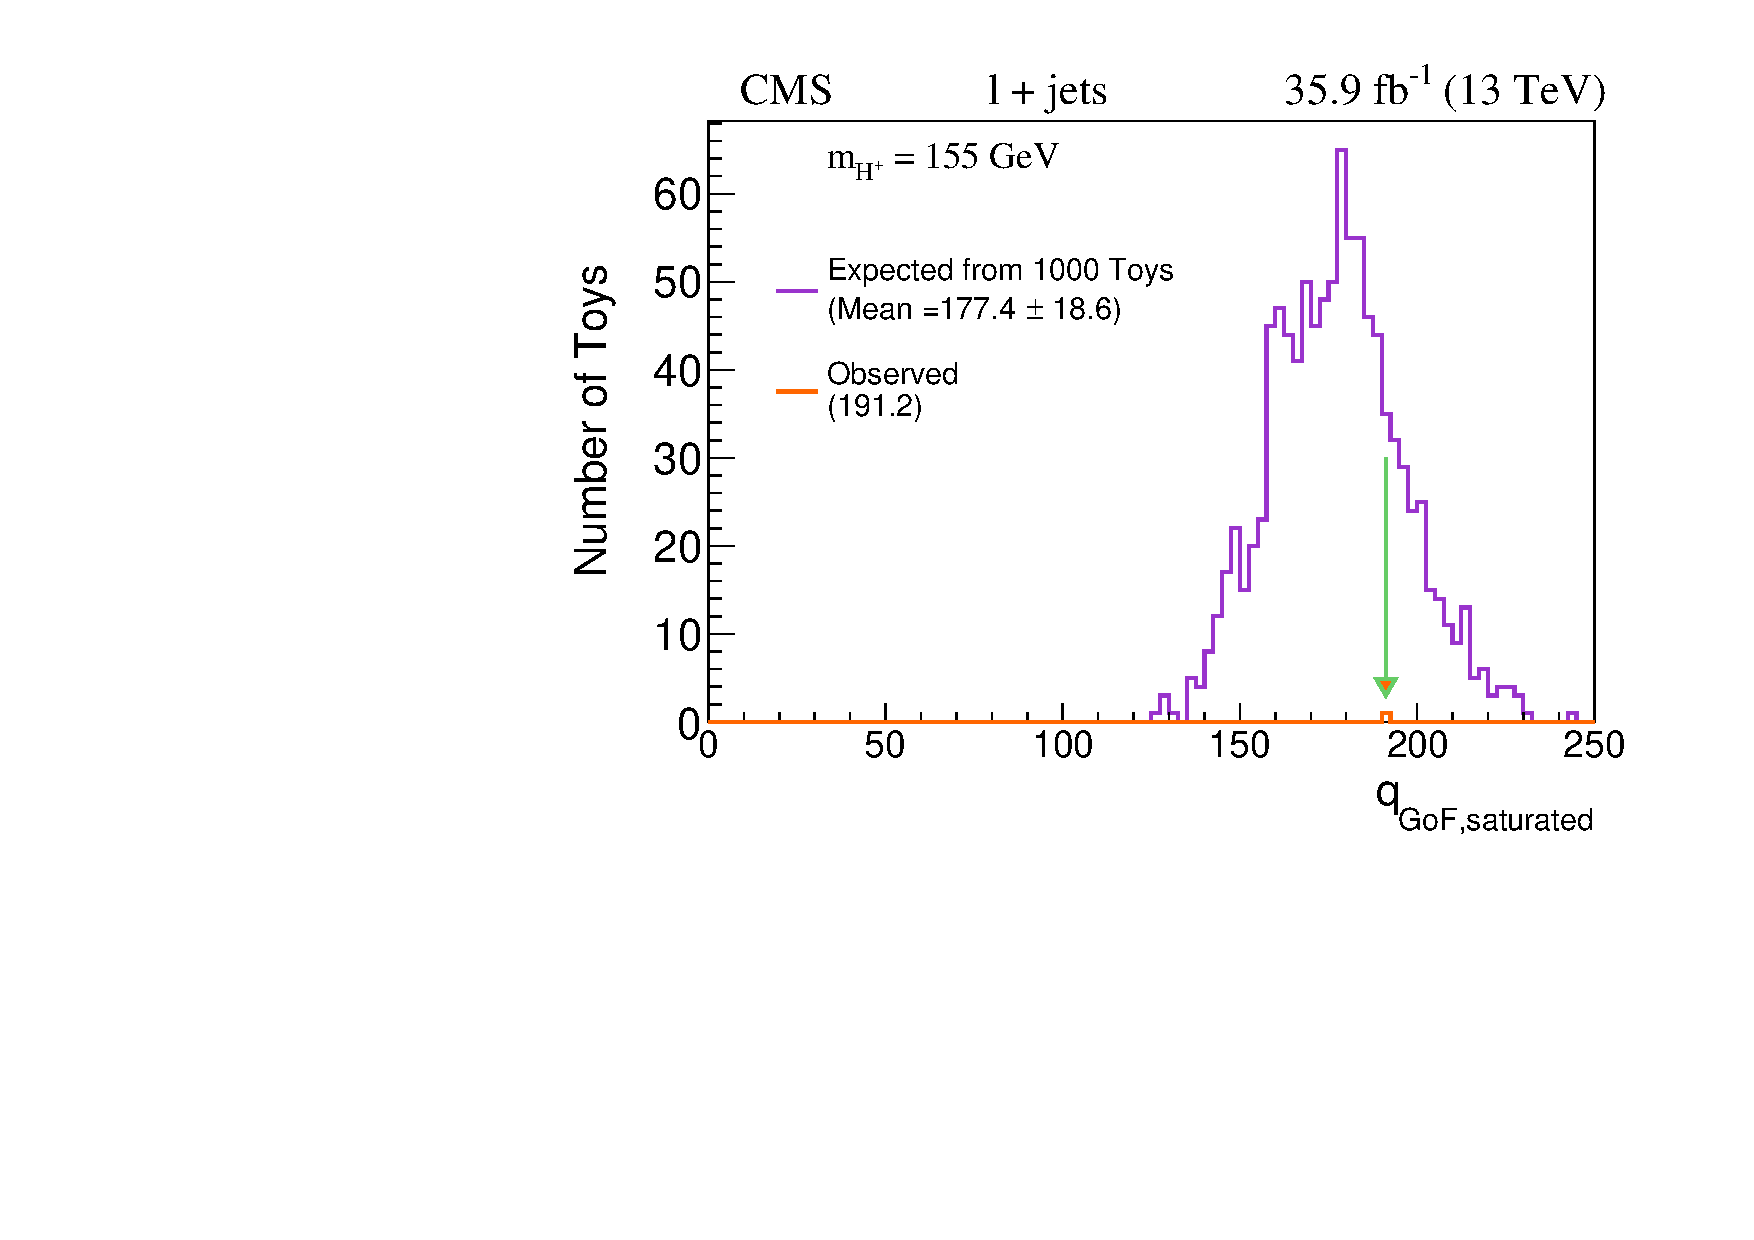
\includegraphics[width=0.45\linewidth]{Image/GOF/GOF_mu_ele_Cat3_cTagEx_155.pdf}}
    \subfigure[]{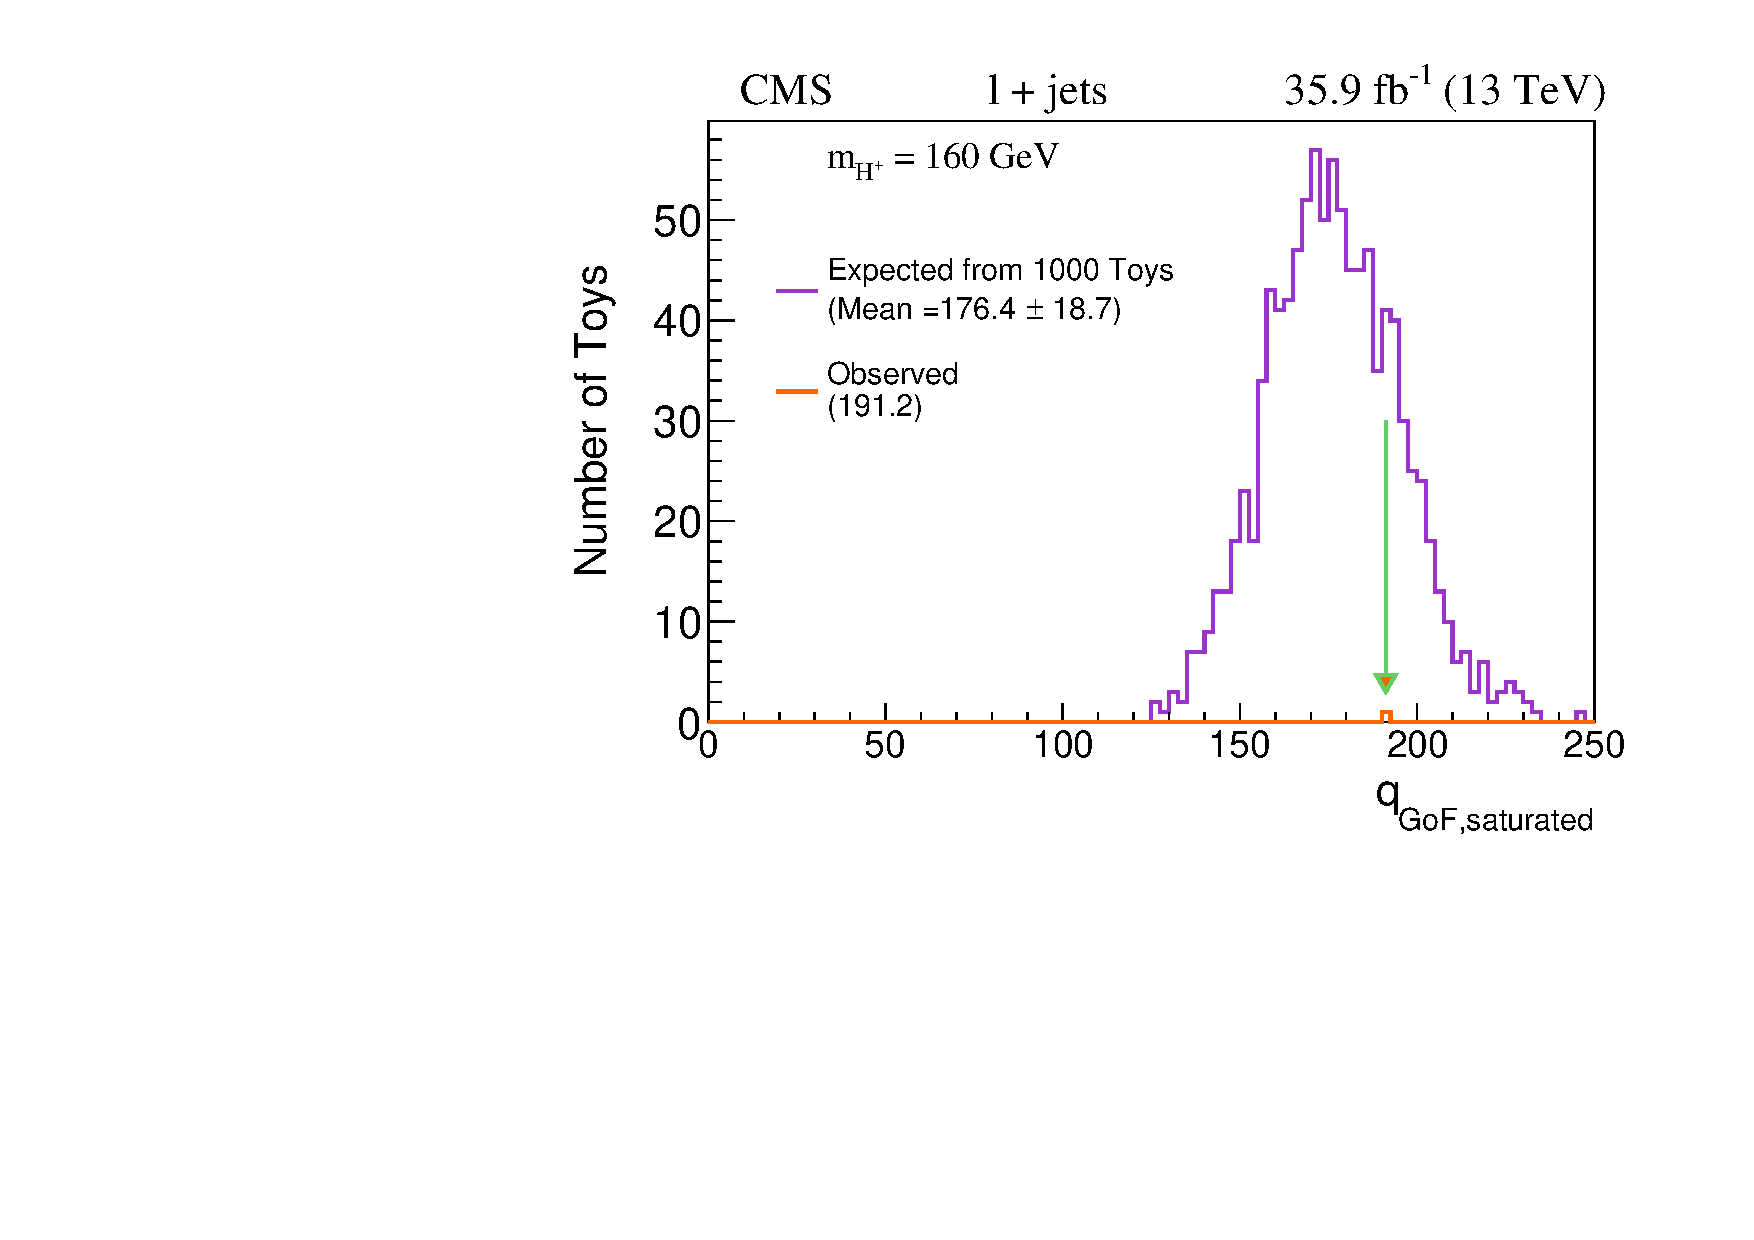
\includegraphics[width=0.45\linewidth]{Image/GOF/GOF_mu_ele_Cat3_cTagEx_160.pdf}}
    \caption{Goodness of fit for lepton channel from exclusive charm categories.}
    \label{fig:GOF}
\end{figure}

\begin{table}
\caption{Goodness of fit for \mujets channel, from different event categories.}
\label{tab:gofMu}
\centering
\begin{adjustbox}{max width=\textwidth}
\begin{tabular}{ ccccccc}
\hline
\hline
\multicolumn{1}{c}{{\bf{$m_{H^\pm}$}}} & \multicolumn{2}{c}{$\mjj(Inc)$} & \multicolumn{2}{c}{$\mjj(Inc ~CTagL)$} & \multicolumn{2}{c}{$\mjj(Ex ~CTag)$} \\

(GeV) & from toys & from data & from toys & from data & from toys & from data  \\
 \hline
\hline
80  & 29.4 $\pm$ 7.5 & 54.4 & 29.7 $\pm$ 7.8 & 56.3 & 89.8 $\pm$ 13.6 & 111.6\\
  
90  & 29.8 $\pm$ 7.6 & 54.4 & 30.0 $\pm$ 8.0 & 56.3 & 89.0 $\pm$ 13.3 & 111.5\\
  
100  & 29.4 $\pm$ 8.3 & 54.4 & 29.4 $\pm$ 7.8 & 56.3 & 89.7 $\pm$ 13.1 & 111.5\\
  
120  & 30.1 $\pm$ 8.2 & 54.4 & 29.4 $\pm$ 7.7 & 56.3 & 89.1 $\pm$ 13.1 & 111.5\\
  
140  & 29.9 $\pm$ 7.7 & 53.2 & 29.4 $\pm$ 7.9 & 56.2 & 90.0 $\pm$ 13.2 & 111.3\\
  
150  & 29.7 $\pm$ 7.8 & 52.6 & 30.0 $\pm$ 7.8 & 55.4 & 89.2 $\pm$ 13.6 & 110.5\\
  
155  & 29.5 $\pm$ 8.2 & 52.2 & 29.6 $\pm$ 8.3 & 54.9 & 89.9 $\pm$ 13.3 & 109.9\\
  
160  & 29.4 $\pm$ 7.6 & 53.7 & 29.3 $\pm$ 8.0 & 55.9 & 89.6 $\pm$ 12.9 & 111.0\\
\hline
\end{tabular}
\end{adjustbox}
\end{table}

\begin{table}
\caption{Goodness of fit for \ejets channel, from different event categories.}
\label{tab:gofEle}
\centering
\begin{adjustbox}{max width=\textwidth}
\begin{tabular}{ ccccccc}
\hline
\hline
\multicolumn{1}{c}{{\bf{$m_{H^\pm}$}}} & \multicolumn{2}{c}{$\mjj(Inc)$} & \multicolumn{2}{c}{$\mjj(Inc ~CTagL)$} & \multicolumn{2}{c}{$\mjj(Ex ~CTag)$} \\

(GeV) & from toys & from data & from toys & from data & from toys & from data  \\
 \hline
\hline
80  & 29.5 $\pm$ 7.4 & 34.1 & 29.6 $\pm$ 7.9 & 34.7 & 89.5 $\pm$ 12.8 & 81.8\\
  
90  & 29.2 $\pm$ 7.7 & 33.1 & 29.2 $\pm$ 7.8 & 34.7 & 88.7 $\pm$ 13.2 & 81.8\\
  
100  & 29.8 $\pm$ 7.6 & 34.1 & 29.8 $\pm$ 7.4 & 34.7 & 89.0 $\pm$ 13.7 & 81.8\\
  
120  & 29.4 $\pm$ 7.5 & 33.8 & 29.2 $\pm$ 7.5 & 34.7 & 89.3 $\pm$ 12.9 & 81.8\\
  
140  & 29.7 $\pm$ 7.9 & 34.1 & 29.3 $\pm$ 7.5 & 34.7 & 89.8 $\pm$ 13.2 & 81.8\\
  
150  & 29.6 $\pm$ 9.1 & 34.1 & 29.0 $\pm$ 7.5 & 34.7 & 88.7 $\pm$ 13.3 & 81.8\\
  
155  & 29.0 $\pm$ 7.3 & 34.1 & 29.4 $\pm$ 7.6 & 34.7 & 89.4 $\pm$ 12.9 & 81.8\\
  
160  & 29.4 $\pm$ 7.4 & 34.1 & 29.4 $\pm$ 7.8 & 34.7 & 89.8 $\pm$ 13.5 & 81.8\\
\hline
\end{tabular}
\end{adjustbox}
\end{table}

\begin{table}
\caption{Goodness of fit for \ljets channel, from different event categories.}
\label{tab:gofLep}
\centering
\begin{adjustbox}{max width=\textwidth}
\begin{tabular}{ ccccccc}
\hline
\hline
\multicolumn{1}{c}{{\bf{$m_{H^\pm}$}}} & \multicolumn{2}{c}{$\mjj(Inc)$} & \multicolumn{2}{c}{$\mjj(Inc ~CTagL)$} & \multicolumn{2}{c}{$\mjj(Ex ~CTag)$} \\

(GeV) & from toys & from data & from toys & from data & from toys & from data  \\
 \hline
\hline
80  & 59.0 $\pm$ 10.8 & 87.0 & 59.0 $\pm$ 11.1 & 89.6 & 173.6 $\pm$ 15.1 & 191.2\\
  
90  & 59.5 $\pm$ 11.1 & 87.0 & 58.5 $\pm$ 10.5 & 89.6 & 173.0 $\pm$ 14.6 & 191.2\\
  
100  & 59.7 $\pm$ 10.5 & 87.0 & 58.7 $\pm$ 10.4 & 89.6 & 173.8 $\pm$ 14.5 & 191.2\\
  
120  & 58.3 $\pm$ 10.3 & 87.0 & 59.5 $\pm$ 10.6 & 89.6 & 173.4 $\pm$ 15.3 & 191.2\\
  
140  & 59.5 $\pm$ 10.9 & 87.0 & 59.5 $\pm$ 10.7 & 89.6 & 173.0 $\pm$ 15.3 & 191.2\\
  
150  & 58.6 $\pm$ 10.2 & 87.0 & 59.4 $\pm$ 10.7 & 89.6 & 173.5 $\pm$ 15.0 & 191.2\\
  
155  & 59.4 $\pm$ 10.5 & 87.0 & 59.0 $\pm$ 10.9 & 89.6 & 173.2 $\pm$ 14.9 & 191.2\\
  
160  & 59.9 $\pm$ 10.8 & 87.0 & 59.8 $\pm$ 10.9 & 89.6 & 172.6 $\pm$ 15.4 & 191.2\\
\hline
\end{tabular}
\end{adjustbox}
\end{table}
